\documentclass{bmstu}

\include{utils}


\usepackage{xcolor}
\usepackage{wrapfig}
\usepackage{upgreek}
\usepackage{pifont}
\newcommand{\cmark}{\ding{51}}%
\newcommand{\xmark}{\ding{55}}%

\definecolor{codegreen}{rgb}{0,0.6,0}
\definecolor{codegray}{rgb}{0.5,0.5,0.5}
\definecolor{codepurple}{rgb}{0.58,0,0.82}
\definecolor{backcolour}{rgb}{0.95,0.95,0.92}

\lstdefinestyle{mystyle}{
	backgroundcolor=\color{backcolour},
	commentstyle=\color{codegreen},
	keywordstyle=\color{magenta},
	numberstyle=\tiny\color{codegray},
	stringstyle=\color{codepurple},
	basicstyle=\ttfamily\footnotesize,
	breakatwhitespace=false,         
	breaklines=true,                 
	captionpos=b,                    
	keepspaces=true,                 
	numbers=left,                    
	numbersep=5pt,                  
	showspaces=false,                
	showstringspaces=false,
	showtabs=false,                  
	tabsize=4,
	emph={trunc, log, histogram, None, plot, xlabel, ylabel, hist, True, mean, std, linspace, norm, pdf, flatten, gamma, as, comb, uniform, sort, transpose, set\_printoptions, seed, zeros},
	emphstyle=\color{magenta}
}

\lstset{style=mystyle}


\usepackage{physics}
\usepackage{pdfpages}
\usepackage{tabularx}
\usepackage{dsfont}
\usepackage{listings}
\usepackage{color}
\usepackage{xfrac}


\graphicspath{
	{graphics/}
}

\begin{document}
	% ТИТУЛЬНИК %
	
	\pagestyle{empty}
	\centerline{\large Министерство науки и высшего образования}	
	\centerline{\large Федеральное государственное бюджетное образовательное}
	\centerline{\large учреждение высшего образования}
	\centerline{\large <<Московский государственный технический университет}
	\centerline{\large имени Н.Э. Баумана}
	\centerline{\large (национальный исследовательский университет)>>}
	\centerline{\large (МГТУ им. Н.Э. Баумана)}
	\hrule
	\vspace{0.5cm}
	\begin{figure}[h]
		\center
		\includegraphics[height=0.30\linewidth]{bmstu-logo.pdf}
	\end{figure}
	\begin{center}
		\large	
		\begin{tabular}{c}
			Факультет <<Фундаментальные науки>> \\
			Кафедра <<Математика и компьютерные науки (ФН11)>>		
		\end{tabular}
	\end{center}
	\vspace{0.5cm}
	\begin{center}
		\LARGE \bf	
		\begin{tabular}{c}
			\textsc{Компьютерная геометрия}
			\\
			\\
			Домашняя работа №1\\ \\
			<<Математические методы, модели и \\
			алгоритмы компьютерной геометрии>> \\
		\end{tabular}
	\end{center}
	\vspace{0.5cm}
	\begin{center}
		\large	
		\begin{tabular}{c}
			Писаревский Арсений -- ФН11-51Б \\ \\
			Преподаватель: Захаров А.А.
		\end{tabular}
	\end{center}
	\vfill
	\begin{center}
		\large	
		\begin{tabular}{c}
			Москва, 
			2023 г.
		\end{tabular}
	\end{center}
	
	% ТИТУЛЬНИК %
	
	\newpage
	
	\section*{Задание:}
	
	Запрограммируйте камеру, пролетающую на высоте 3 единицы над последовательностью мячей, расположенных вдоль оси $x$, которая направлена вперед и вниз на мячи.
	
	\begin{figure}[H]
		\centering
		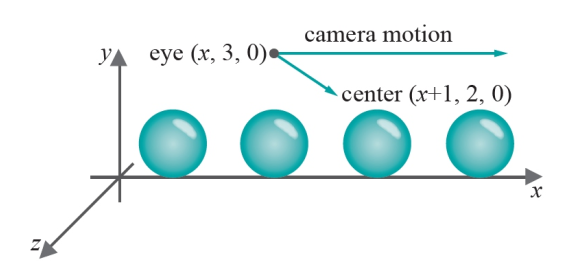
\includegraphics[width=0.8\linewidth]{graphics/camera}
		\caption{Камера, пролетающая над мячами}
		\label{fig:camera}
	\end{figure}
	
	
	\section*{Код программы:}
	
	\section*{Вывод:}
	
	
\end{document}